\documentclass{beamer}
\usetheme{default}
\beamertemplatenavigationsymbolsempty
\usepackage{rembeamer}

\begin{document}

\begin{frame}
  \begin{itemize}
    \item[] 
      LO4: Interpret various visualizations of categorical data:
      bar plots, mosaic plots, and pie charts.
  \end{itemize}
\end{frame}

\begin{frame}
  \frametitle{Frequency Table}
  \centering
  \begin{table}
    \begin{tabular}{@{}cc@{}}
      \toprule
      Ownership & Count \\
      \cmidrule(r){1-1} \cmidrule(l){2-2} 
      Mortgage & 4789 \\
      Own & 1353 \\
      Rent & 3858 \\
      \cmidrule(r){1-1} \cmidrule(l){2-2} 
      Total & 100000 \\
      \bottomrule 
    \end{tabular}
  \end{table}
\end{frame}

\begin{frame}
  \frametitle{Bar Plot - Ownership Variable}
  \centering
  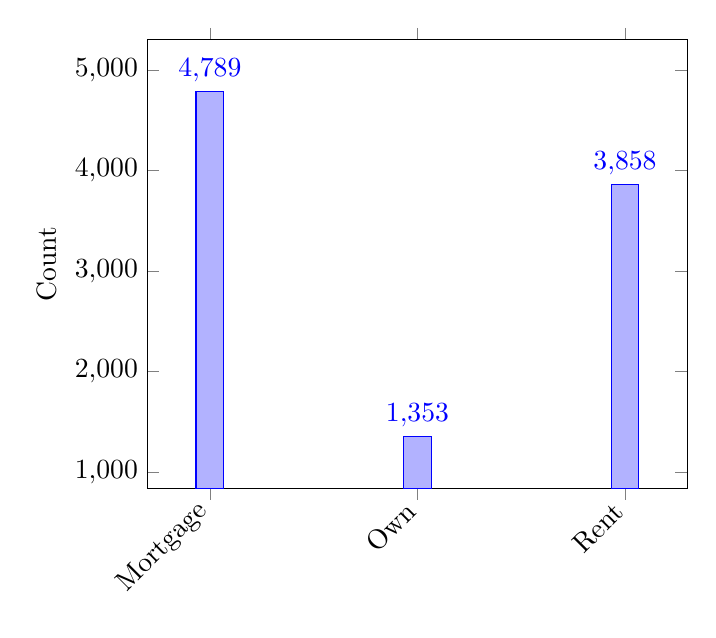
\begin{tikzpicture}
    \begin{axis}[
      ybar,
      enlargelimits=0.15,
      legend style={at={(0.5,-0.2)},
      anchor=north,legend columns=-1},
      ylabel={Count},
      symbolic x coords={Mortgage,Own,Rent},
      xtick=data,
      nodes near coords,
      nodes near coords align={vertical},
      x tick label style={rotate=45,anchor=east},
    ]
    \addplot coordinates {
      (Mortgage,4789) (Own,1353) (Rent,3858)
    };
  \end{axis}
  \end{tikzpicture}
\end{frame}

\begin{frame}
  \frametitle{Bar Plot - Ownership Variable Proportions}
  \centering
  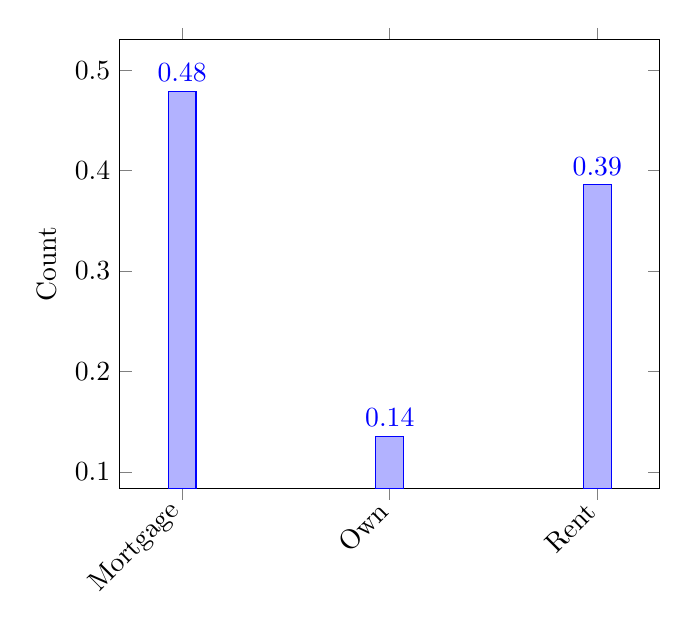
\begin{tikzpicture}
    \begin{axis}[
      ybar,
      enlargelimits=0.15,
      legend style={at={(0.5,-0.2)},
      anchor=north,legend columns=-1},
      ylabel={Count},
      symbolic x coords={Mortgage,Own,Rent},
      xtick=data,
      nodes near coords,
      nodes near coords align={vertical},
      x tick label style={rotate=45,anchor=east},
    ]
    \addplot coordinates {
      (Mortgage,0.4789) (Own,0.1353) (Rent,0.3858)
    };
  \end{axis}
  \end{tikzpicture}
\end{frame}

\begin{frame}
  \frametitle{Contingency Table}
  \centering
  \begin{table}
    \begin{tabular}{@{}cccc@{}}
      \toprule
      Ownership & Individual & Joint & Total  \\
      \cmidrule(r){1-1} \cmidrule(rl){2-4} \cmidrule(rl){3-3}
      \cmidrule(l){4-4}
      Mortgage & 3977 & 812 & 4789 \\
      Own & 1242 & 111 & 1353 \\ 
      Rent & 3494  & 364 & 3858 \\
      \cmidrule(r){1-1} \cmidrule(rl){2-4} \cmidrule(l){3-3}
      \cmidrule(l){4-4}
      Total & 8713 & 1287 & 100000 \\
      \bottomrule 
    \end{tabular}
  \end{table}
\end{frame}

\begin{frame}
  \frametitle{Stacked Bar Plot - Ownership by Application Type}
  \centering
  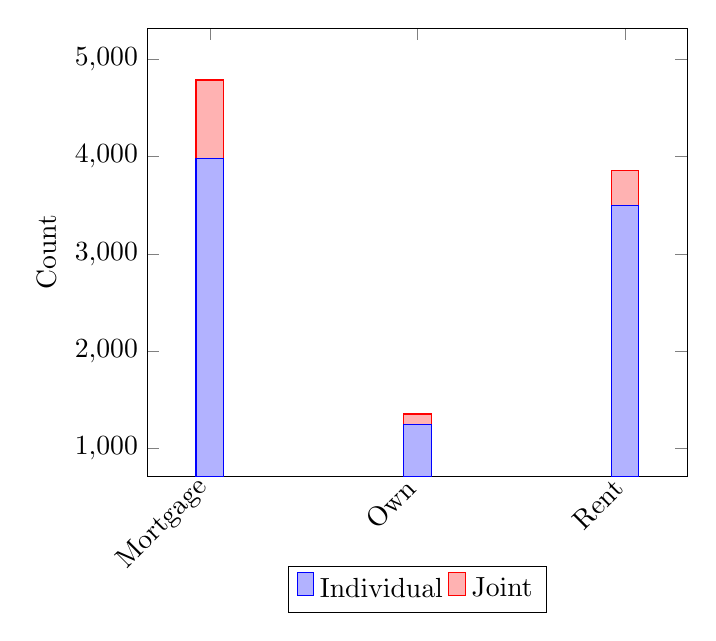
\begin{tikzpicture}
    \begin{axis}[
      ybar stacked,
      enlargelimits=0.15,
      legend style={at={(0.5,-0.2)},
      anchor=north,legend columns=-1},
      ylabel={Count},
      symbolic x coords={Mortgage,Own,Rent},
      xtick=data,
      x tick label style={rotate=45,anchor=east},
    ]
    \addplot+ [ybar] coordinates {(Mortgage,3977) (Own,1242)
    (Rent,3494)};
    \addplot+ [ybar] coordinates {(Mortgage,812) (Own,111)
    (Rent,364)};
    \legend{Individual,Joint}
  \end{axis}
  \end{tikzpicture}
\end{frame}

\begin{frame}
  \frametitle{Dodged Bar Plot - Ownership by Application Type}
  \centering
  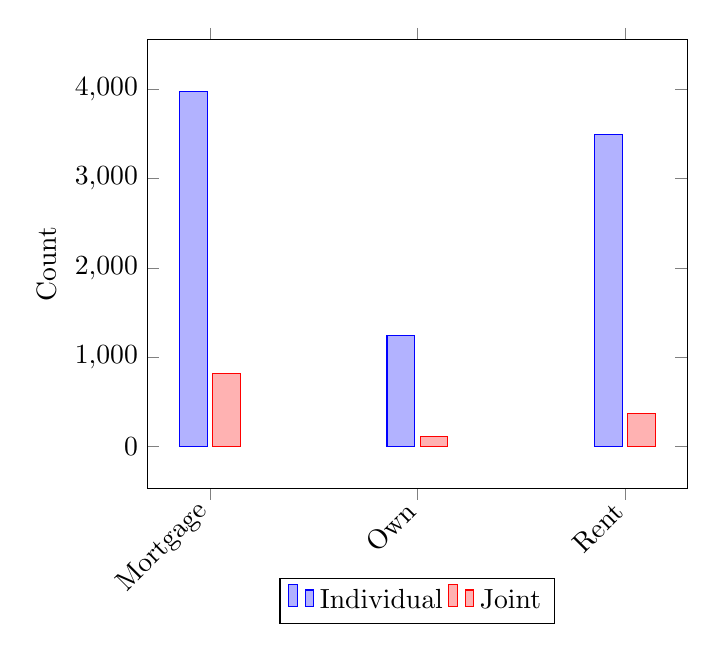
\begin{tikzpicture}
    \begin{axis}[
      ybar,
      enlargelimits=0.15,
      legend style={at={(0.5,-0.2)},
      anchor=north,legend columns=-1},
      ylabel={Count},
      symbolic x coords={Mortgage,Own,Rent},
      xtick=data,
      x tick label style={rotate=45,anchor=east},
    ]
    \addplot coordinates {(Mortgage,3977) (Own,1242)
    (Rent,3494)};
    \addplot coordinates {(Mortgage,812) (Own,111)
    (Rent,364)};
    \legend{Individual,Joint}
  \end{axis}
  \end{tikzpicture}
\end{frame}

\begin{frame}
  \frametitle{Standardized Bar Plot - Ownership by Application Type}
  \centering
  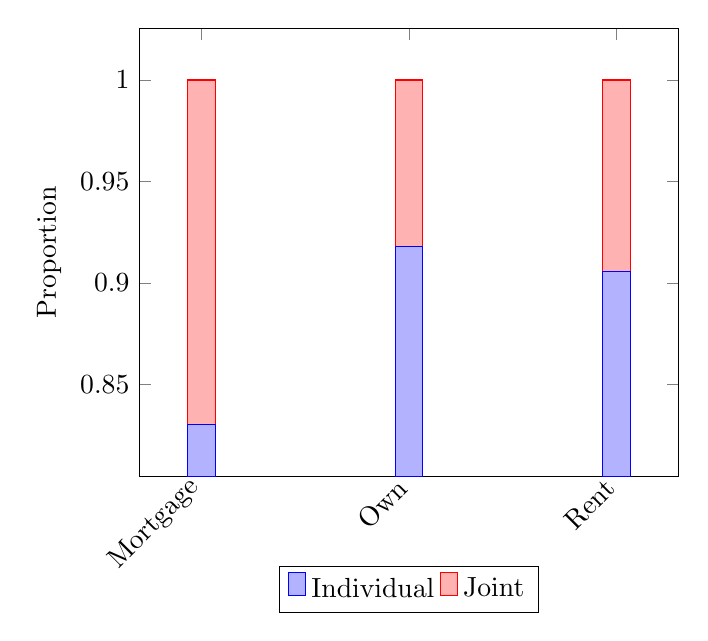
\begin{tikzpicture}
    \begin{axis}[
      ybar stacked,
      enlargelimits=0.15,
      legend style={at={(0.5,-0.2)},
      anchor=north,legend columns=-1},
      ylabel={Proportion},
      symbolic x coords={Mortgage,Own,Rent},
      xtick=data,
      x tick label style={rotate=45,anchor=east},
    ]
    \addplot+ [ybar] coordinates {(Mortgage,0.83) (Own,0.918)
    (Rent,0.9057)};
    \addplot+ [ybar] coordinates {(Mortgage,0.17) (Own,0.082)
    (Rent,0.0943)};
    \legend{Individual,Joint}
  \end{axis}
  \end{tikzpicture}
\end{frame}

\begin{frame}
  \frametitle{Pie Chart - Ownership Variable}
  \centering
  \begin{tikzpicture}
    \pie{47.89/Mortgage,
      13.53/Own,
      38.58/Rent}
  \end{tikzpicture}
\end{frame}

\begin{frame}
  \frametitle{Pie Chart - Loan Grade Variable}
  \centering
  \begin{tikzpicture}
    \pie{24.3/A,
      32.5/B,
      26.2/C,
      11.5/D,
      4.0/E,
      0.9/F,
      0.6/G}
  \end{tikzpicture}
\end{frame}
\end{document}
